% cd /storage/emulated/0/Documents/documents/latex/1920/Grade-8/2nd/theorems-on-perpendicular-lines && pdflatex ps-theorems-on-perpendicular-lines.tex && termux-open ps-theorems-on-perpendicular-lines.pdf

% cd /storage/emulated/0/Documents/documents/latex/1920/Grade-8/2nd/theorems-on-perpendicular-lines && clean-tex ps-theorems-on-perpendicular-lines-input1.tex


% cd /storage/emulated/0/Documents/documents/latex/1920/Grade-8/2nd/theorems-on-perpendicular-lines && convert -density 600 ps-theorems-on-perpendicular-lines.pdf -crop 2200x1700 -quality 100 -verbose ps-theorems-on-perpendicular-lines%02d.png

%2480.5x3508 portrait 2x2 2550x3300
%3508x2480.5 landscape 2x2 3300x2550 
%1653.7x2338.7 portrait 3x3 1700x2200
%landscape 3x3 2200x1700

% cd /storage/emulated/0/Documents/documents/latex/1819/grade10/visual/4th/theorems-on-perpendicular-lines && while inotifywait -e close_write ps-theorems-on-perpendicular-lines*.tex; do touch /storage/emulated/0/Android/data/com.termux/files/launch-termux.txt && printf '1' > /storage/emulated/0/Android/data/com.termux/files/launch-termux.txt && pdflatex ps-theorems-on-perpendicular-lines.tex && termux-open ps-theorems-on-perpendicular-lines.pdf; done

% cd /host-rootfs/storage/emulated/0/Documents/documents/latex/1819/grade10/visual/4th/theorems-on-perpendicular-lines && while inotifywait -e close_write ps-theorems-on-perpendicular-lines*.tex; do pdflatex ps-theorems-on-perpendicular-lines.tex  && printf "/storage/emulated/0/Documents/documents/latex/1819/grade10/visual/4th/theorems-on-perpendicular-lines/ps-theorems-on-perpendicular-lines.pdf" > /host-rootfs/storage/emulated/0/GNURoot/home/Scripts/file-to-launch.txt; done


\documentclass[10pt]{article}
\usepackage[letterpaper, landscape, right=0.25in, left=0.4in, top=0.25in, bottom=0.25in]{geometry}
\usepackage{xcolor}
\usepackage{anyfontsize}
\usepackage{enumitem}
\usepackage{multicol}
\usepackage{bm} 
\usepackage{amsmath}
%\usepackage{amsfonts,dsfont}% for \mathds 
\usepackage{tabularx} 
\usepackage{gensymb}
\usepackage{multirow}
\usepackage{graphicx, tipa}
\usepackage{tikz}
\usetikzlibrary{angles,quotes}
\usepackage{pgfplots} 
\usetikzlibrary{calc}
\pgfplotsset{compat=newest}
\usetikzlibrary{arrows.meta}
\usetikzlibrary{intersections}
\usetikzlibrary{decorations.pathreplacing}
\usepackage{flafter}
\usepackage{amsmath,amssymb,cancel,units}
\usepackage{microtype} % nicer output 
\usepackage{hfoldsty} % nicer output 
\usepackage{fixltx2e} 
\usepackage{mathptmx}
%\usepackage{booktabs}
\usepackage{numprint}
\usepackage[utf8]{inputenc} 
\usepackage[T1]{fontenc}
%\usepackage{siunitx} 
%\sisetup{detect-all}
\usepackage{stackengine}
 
\newcommand\pesos{\stackengine{-1.28ex}{P}{\stackengine{-1.2ex}{$-$}{$-$}{O}{c}{F}{F}{S}}{O}{c}{F}{T}{S}} 


\def\radA{3.6cm}

\def\radB{3.6cm}

%\def\thirdrad{8cm}

\pagenumbering{gobble}
%\linespread{0.9}
\newcommand{\vspce}{\vspace{0.75ex}}
\newcommand{\hspce}{\hspace{0.5em}}
\newcommand{\blank}{\underline{\hspace{2em}}}%{\rule{1em}{0.15ex}}
\newcommand{\arc}[1]{{% 
\setbox9=\hbox{#1}% 
\ooalign{\resizebox{\wd9}{\height}{\texttoptiebar{\phantom{A}}}\cr#1}}}

\newcolumntype{C}{ >{\centering\arraybackslash} X}




\begin{document}
\boldmath
{\fontsize{37}{39}\fontfamily{pnc}\selectfont {

\textbf{Practice Exercises}

\vspce

The adjoining figure consists of 3 coplanar lines passing through $O$ with $\overline{AB} \perp \overline{CD}$. Determine each statement as true or false.

%\begin{center}
%\vspace*{2ex}
%\scalebox{1}{
%\noindent\begin{minipage}{\textwidth}
{\begin{enumerate}[label = \arabic*. ]
%\begin{multicols}{2}
%1
\item	$m\angle{AOC}=90\degree$ 
\item	$m\angle{FOD}= m\angle{AOD} - m\angle{AOF}$ 
\item	$\angle{COF}$ is an acute angle
\item	$\overleftrightarrow{EF} \perp \overleftrightarrow{CD}$ 
\item	$\overrightarrow{OC}$ and $\overrightarrow{OF}$ are opposite rays 
\item	$\angle{AOF}$ and $\angle{AOD}$ are adjacent angles
\item	$\angle{AOD}$ is a right angle
\item	$\angle{AOC}$ and $\angle{AOD}$ are congruent\\ adjacent supplementary angles.
\item	The exterior sides of $\angle{AOF}$ and $\angle{FOD}$ lie in perpendicular lines.
\item	$\overrightarrow{OB} \perp \overrightarrow{OD} $
%\end{multicols} 
\end{enumerate}}
%\end{minipage}}
%\end{center}  

\vspace*{-14.5em}\hspace*{18em}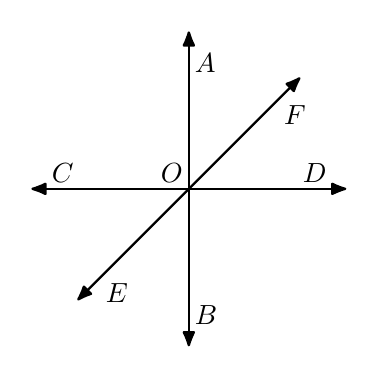
\begin{tikzpicture}

\coordinate (O) at (0,0);

\node[anchor=south east, inner sep=2pt, rotate=0] (O-label) at (O) {$O$}; 

\foreach \ang/\label/\dir in {0/D/south,45/F/north west,90/A/west,180/C/south,225/E/north west,270/B/west} {

\coordinate (\label) at ($(O) + (\ang:2cm)$); 

\draw[line width=0.3mm, ->, >={Latex[round]}] (O) -- (\label);  

\node[anchor=\dir, inner sep=2pt, rotate=0] (label-\label) at ($(O)+ (\ang:1.6cm)$) {$\label$};
}

\end{tikzpicture} 
 
\vspace*{2em}


     







%}} 

\newpage

%{\fontsize{38}{40}\fontfamily{pnc}\selectfont {

\input{ps-theorems-on-perpendicular-lines-input2}

\newpage

%{\fontsize{38}{40}\fontfamily{pnc}\selectfont {

\textbf{Problem Set}

\vspce

The adjoining figure consists of 3 coplanar lines passing through $O$ with $\overline{AL} \perp \overline{UB}$. Determine each statement as true or false.

%\begin{center}
%\vspace*{2ex}
%\scalebox{1}{
%\noindent\begin{minipage}{\textwidth}
{\begin{enumerate}[label = \arabic*. ]
%\begin{multicols}{2}
%1
\item	$m\angle{AOB}=90\degree$ 
\item	$m\angle{KOU}= m\angle{AOU} - m\angle{AOK}$ 
\item	$\angle{KOB}$ is an acute angle
\item	$\overleftrightarrow{KW} \perp \overleftrightarrow{UB}$ 
\item	$\overrightarrow{OB}$ and $\overrightarrow{OK}$ are opposite rays 
\item	$\angle{AOK}$ and $\angle{AOU}$ are adjacent angles
\item	$\angle{AOU}$ is a right angle
\item	$\angle{AOB}$ and $\angle{AOU}$ are congruent\\ adjacent supplementary angles.
\item	The exterior sides of $\angle{AOK}$ and $\angle{KOU}$ lie in perpendicular lines.
\item	$\overrightarrow{OL} \perp \overrightarrow{OU} $
%\end{multicols} 
\end{enumerate}}
%\end{minipage}}
%\end{center}  

\vspace*{-14.5em}\hspace*{18em}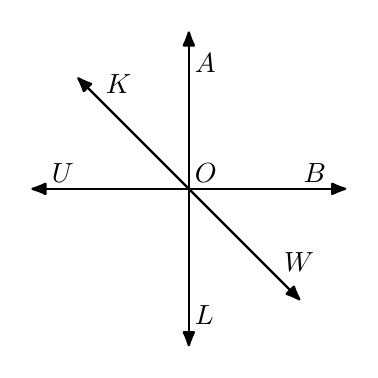
\begin{tikzpicture}

\coordinate (O) at (0,0);

\node[anchor=south west, inner sep=2pt, rotate=0] (O-label) at (O) {$O$}; 

\foreach \ang/\label/\dir in {0/B/south,90/A/west,135/K/south west,180/U/south,270/L/west,315/W/south west} {

\coordinate (\label) at ($(O) + (\ang:2cm)$); 

\draw[line width=0.3mm, ->, >={Latex[round]}] (O) -- (\label);  

\node[anchor=\dir, inner sep=2pt, rotate=0] (label-\label) at ($(O)+ (\ang:1.6cm)$) {$\label$};
}

\end{tikzpicture} 
 
\vspace*{2em}


     







}}

\newpage

{\fontsize{35}{38}\fontfamily{pnc}\selectfont {

\input{ps-theorems-on-perpendicular-lines-sol}

}}


\end{document}